%%%%%%%%%%%%%%%%%%%%%%%%%%%%%%%%%%%%%%%%%
% Beamer Presentation
% LaTeX Template
% Version 1.0 (10/11/12)
%
% This template has been downloaded from:
% http://www.LaTeXTemplates.com
%
% License:
% CC BY-NC-SA 3.0 (http://creativecommons.org/licenses/by-nc-sa/3.0/)
%
%%%%%%%%%%%%%%%%%%%%%%%%%%%%%%%%%%%%%%%%%

%----------------------------------------------------------------------------------------
%	PACKAGES AND THEMES
%----------------------------------------------------------------------------------------

\documentclass{beamer}

\mode<presentation> {

% The Beamer class comes with a number of default slide themes
% which change the colors and layouts of slides Below this is a list
% of all the themes, uncomment each in turn to see what they look like.

%\usetheme{default}
%\usetheme{AnnArbor}
%\usetheme{Antibes}
%\usetheme{Bergen}
%\usetheme{Berkeley}
%\usetheme{Berlin}
%\usetheme{Boadilla}
%\usetheme{CambridgeUS}
%\usetheme{Copenhagen}
%\usetheme{Darmstadt}
%\usetheme{Dresden}
%\usetheme{Frankfurt}
%\usetheme{Goettingen}
%\usetheme{Hannover}
%\usetheme{Ilmenau}
%\usetheme{JuanLesPins}
%\usetheme{Luebeck}
\usetheme{Madrid}
%\usetheme{Malmoe}
%\usetheme{Marburg}
%\usetheme{Montpellier}
%\usetheme{PaloAlto}
%\usetheme{Pittsburgh}
%\usetheme{Rochester}
%\usetheme{Singapore}
%\usetheme{Szeged}
%\usetheme{Warsaw}

% As well as themes, the Beamer class has a number of color themes
% for any slide theme Uncomment each of these in turn to see how it
% changes the colors of your current slide theme.

%\usecolortheme{albatross}
%\usecolortheme{beaver}
%\usecolortheme{beetle}
%\usecolortheme{crane}
%\usecolortheme{dolphin}
%\usecolortheme{dove}
%\usecolortheme{fly}
%\usecolortheme{lily}
%\usecolortheme{orchid}
%\usecolortheme{rose}
%\usecolortheme{seagull}
%\usecolortheme{seahorse}
%\usecolortheme{whale}
%\usecolortheme{wolverine}

%\setbeamertemplate{footline} % To remove the footer line in all slides uncomment this line
%\setbeamertemplate{footline}[page number] % To replace the footer line in all slides with a simple slide count uncomment this line

%\setbeamertemplate{navigation symbols}{} % To remove the navigation symbols from the bottom of all slides uncomment this line
}

\usepackage{graphicx} % Allows including images
\usepackage{booktabs} % Allows the use of \toprule, \midrule and \bottomrule in tables
\usepackage{multicol}

\let\cross\times
\let\vec\boldsymbol

%----------------------------------------------------------------------------------------
%	TITLE PAGE
%----------------------------------------------------------------------------------------

\title[Thesis Presentation]{Jens Edhammer Thesis Presentation} % The short title appears at the bottom of every slide, the full title is only on the title page

\author{Jens Edhammer} % Your name
\institute[LiU] % Your institution as it will appear on the bottom of every slide, may be shorthand to save space
{
Link\"{o}pings Universitet \\ % Your institution for the title page
\medskip
\textit{} % Your email address
}
\date{June 2016} % Date, can be changed to a custom date



\begin{document}

	\begin{frame}
		\titlepage % Print the title page as the first slide
	\end{frame}

	\begin{frame}<beamer>
		\begin{multicols}{2}
			\frametitle{Overview}
			\tableofcontents
		\end{multicols}
	\end{frame}

	%----------------------------------------------------------------------------------------
	%	PRESENTATION SLIDES
	%----------------------------------------------------------------------------------------

	%------------------------------------------------
	\section{Problem Description} % Sections can be created in order to organize your presentation into discrete blocks, all sections and subsections are automatically printed in the table of contents as an overview of the talk
	%------------------------------------------------

	%Collision detection and resolution of approximately concave objects, preferably fast
	\subsection{Purpose}
	%To be used to simulate the part distribution in the PLB system
	\begin{frame}
		\frametitle{Purpose}
		Using rigid body physics we aim to generate synthetic data
		\begin{figure}
			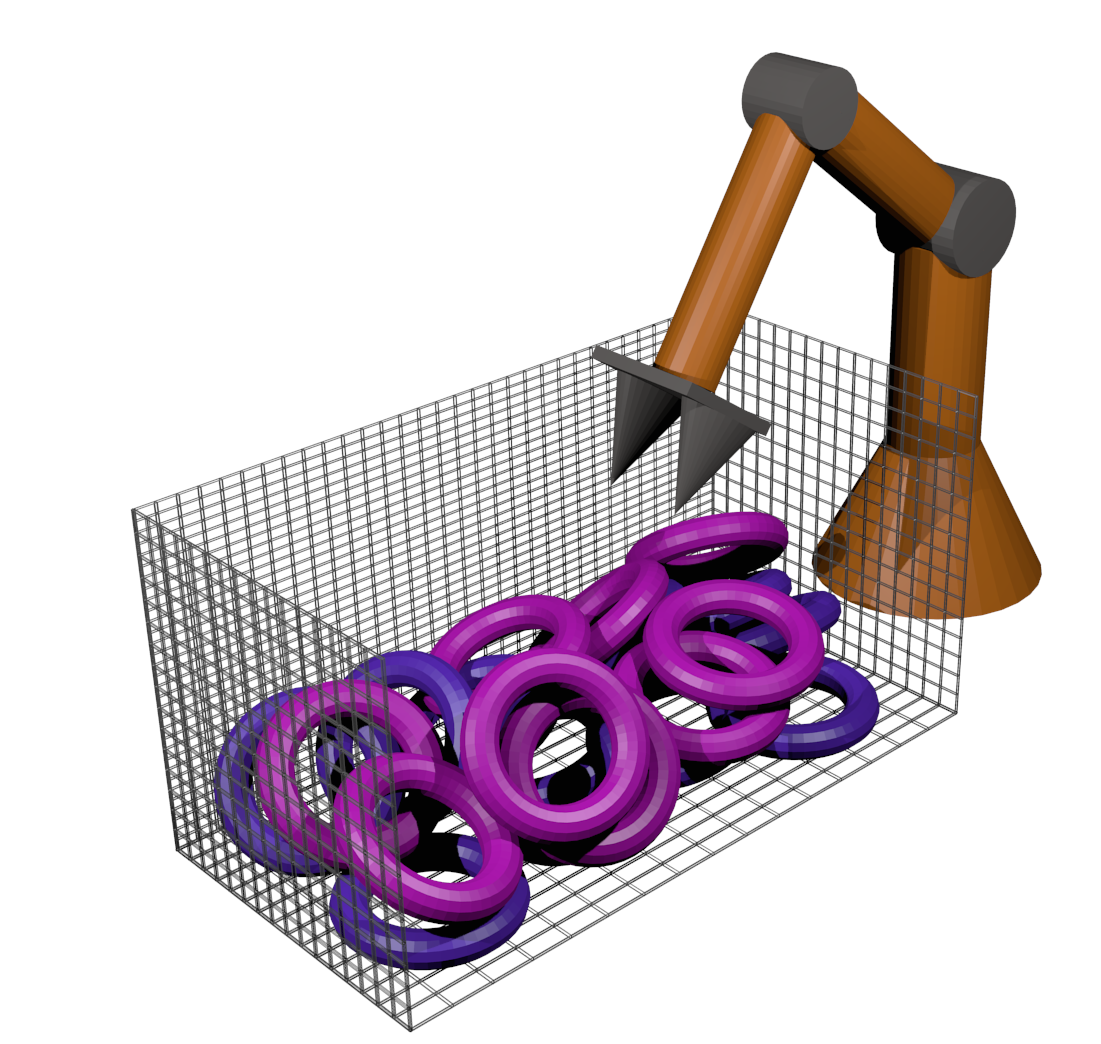
\includegraphics[width=0.6\linewidth]{fig/binBlender.png}
		\end{figure}
	\end{frame}

	\subsection{Method}
	\begin{frame}
		\frametitle{Method}
		The thesis compares Bullet 2.83 against a new GPU solution \\
		The points of interests are
		\begin{itemize}
			\item Performance
			\item Concave collision shapes
			\item Physical plausibility
		\end{itemize}
		The first is compared between the two solutions while the second two are more or less a yes or no question
	\end{frame}
	%Comparison between Bullet (established solution) and impulse based spherical voxelization (Sphox)
	%Of interest is performance, concave properties and physical plausibility of the distribution.
	\AtBeginSection[2]
	{
	\begin{frame}<beamer>
		\begin{multicols}{2}
			\frametitle{Plan}
			\tableofcontents[currentsection, hideothersubsections]
		\end{multicols}
	\end{frame}
	}

	\section{Bullet}
	\begin{frame}
		\frametitle{Bullet 2.86}
		Physics library running on the CPU\\
		Distributed under a permissive open source license
	\end{frame}
	\subsection{HACD}
	\begin{frame}
		\frametitle{HACD}
		HACD - Heirarchical Approximate Convex Decomposition \\
		Method for automatic Convex Decomposition of models
		\begin{figure}
			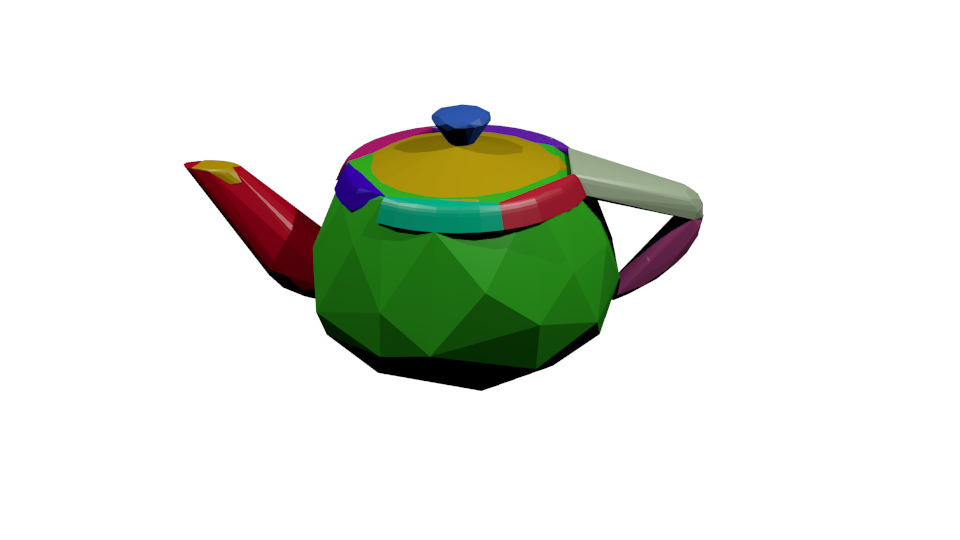
\includegraphics[width=0.5\linewidth]{fig/hacdTeapot.png}
		\end{figure}
	\end{frame}

	\begin{frame}
		\frametitle{Results}
		Good results with concave properties and decent performance
		\begin{figure}
			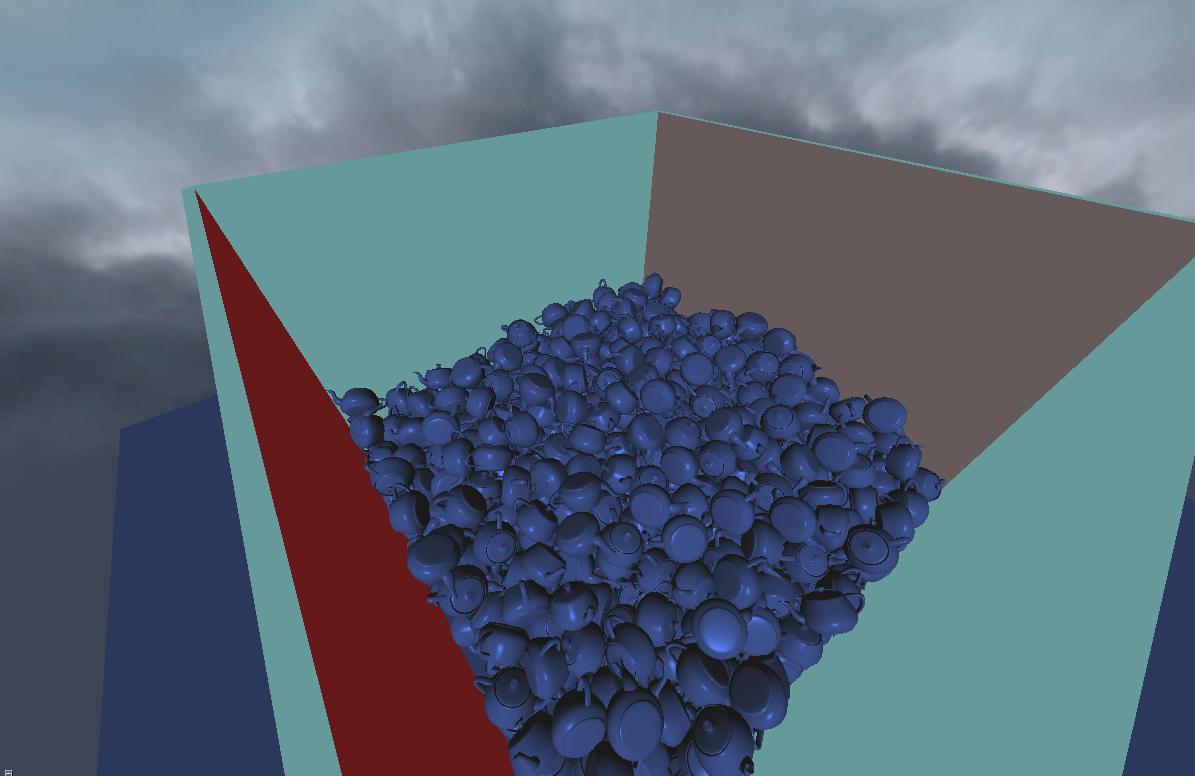
\includegraphics[width=0.7\linewidth]{fig/HACD512-05-11.png}
		\end{figure}
	\end{frame}

	%
	%	How do we get concave results? Voxelization
	%
	\section{Impulses on the GPU}
	\subsection{Spherical Voxelization}
	\begin{frame}
		\frametitle{Spherical Voxelization}
		%\begin{columns}[c] % The "c" option specifies centered vertical alignment while the "t" option is used for top vertical alignment
		%	\column{.45\textwidth} % Left column and width
		Instead of using different submodels we can decompose a model into only spheres (or particles)
		%	\column{.5\textwidth} % Right column and width
		\begin{figure}
			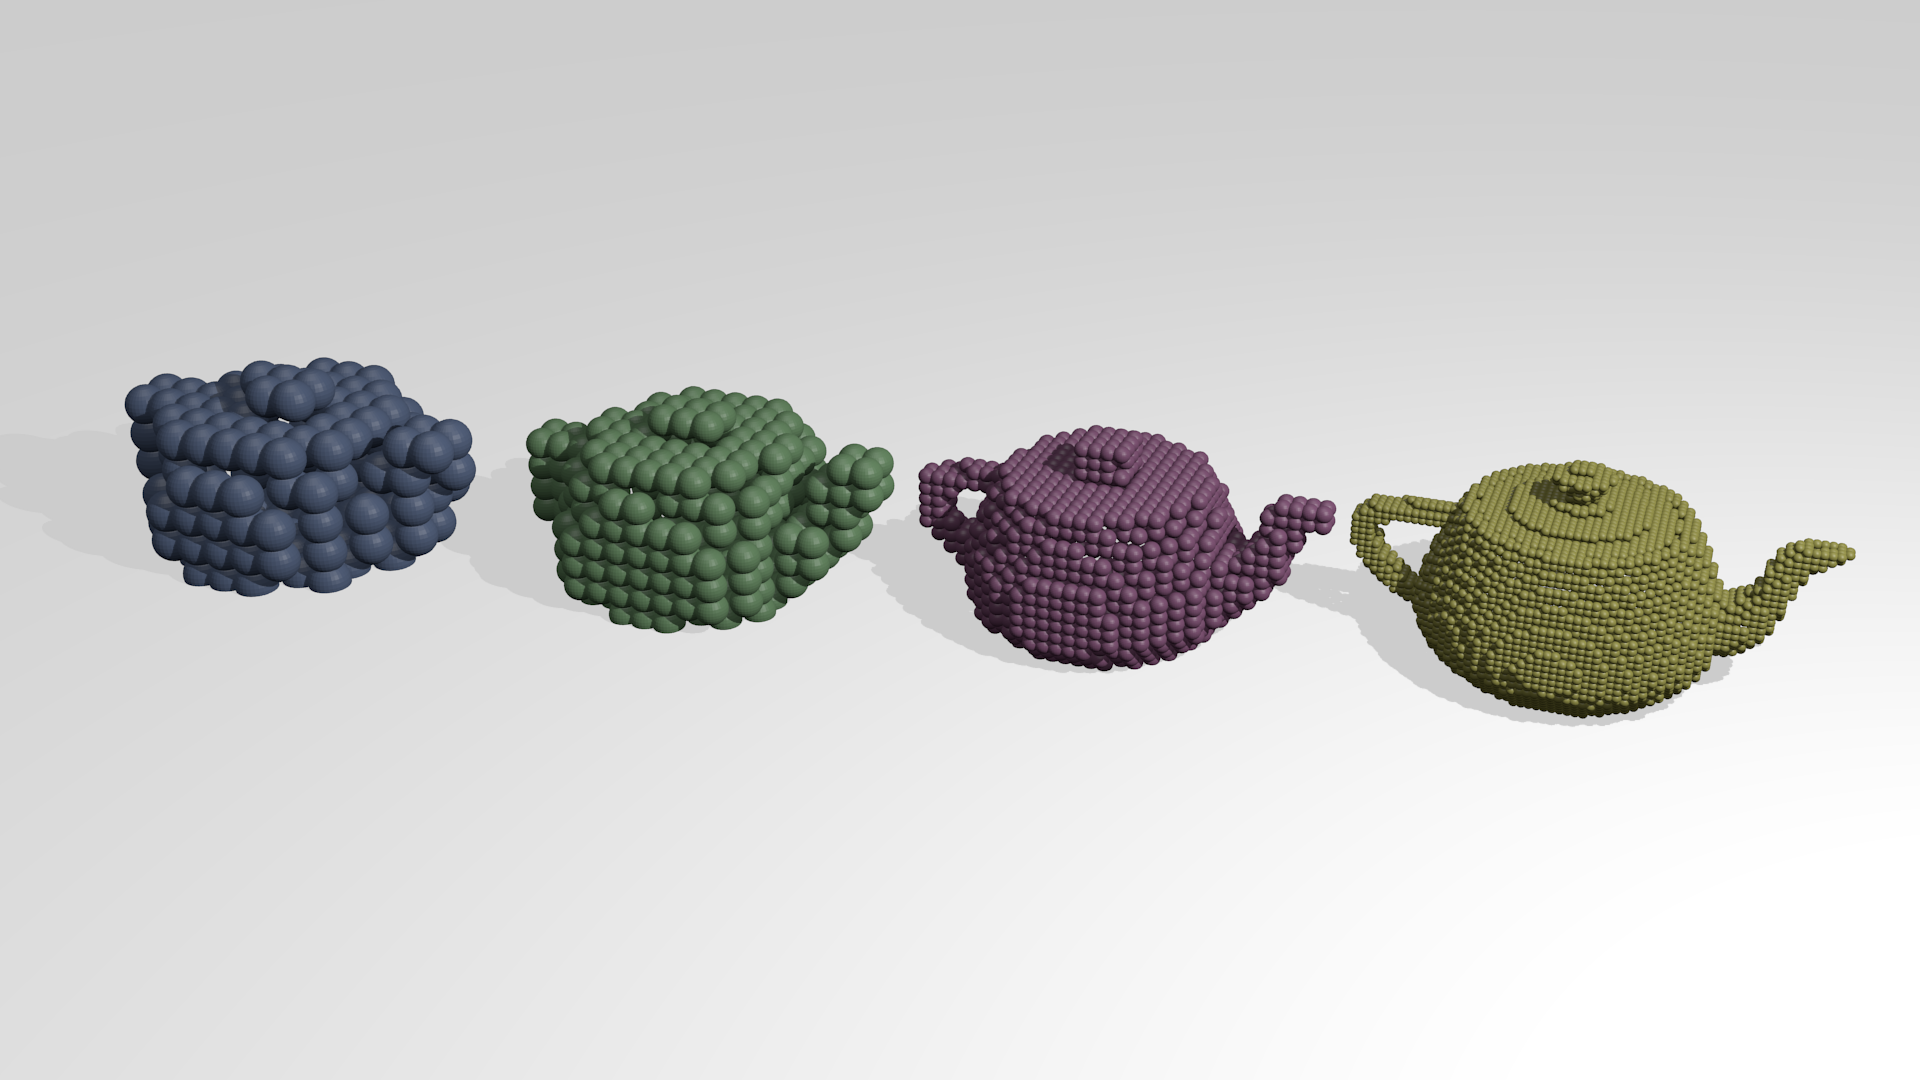
\includegraphics[width=0.8\linewidth]{fig/voxelExample.png}
		\end{figure}
		%	\end{columns}
	\end{frame}

	%
	%	Benefits of using a single shape
	%
	\begin{frame}
		\frametitle{Spherical Voxelization}
		Benefits from using a single subshape:
		\begin{itemize}
			\item Concave collision properties
			\item All bodies handled the same way
			\item Suitable for GPU implementations
		\end{itemize}
	\end{frame}

	%
	%	Description of spring dampner.
	%
	\subsection{Physics}

	\begin{frame}
		\frametitle{Spring-Dampner system}
		\begin{itemize}
			\item Previous work by nvidia present a spring-dampner system
			\item Each particle collision modeled as a spring and a dampner
			\item While fast it has drawbacks in how to stabilize the system
		\end{itemize}
	\end{frame}
	%
	%Description of Impulse Physics
	%
	\begin{frame}
		\frametitle{Impulse Physics}
		\begin{columns}[c] % The "c" option specifies centered vertical alignment while the "t" option is used for top vertical alignment
			\column{.45\textwidth} % Left column and width
			Instead use impulses from rigid body mechanics
			When two items collide an impulse is created between them
			\column{.5\textwidth} % Right column and width

			\begin{figure}
				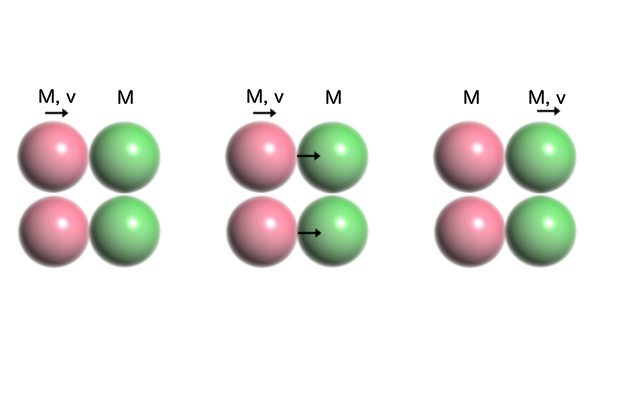
\includegraphics[width=0.8\linewidth]{fig/ballsExpected.png}
			\end{figure}

		\end{columns}
	\end{frame}

	%
	%Description of j
	%

	\begin{frame}
		\frametitle{Impulse Physics}
		The math is presented in an easily approached form by David Baraff
		The impulse which need to be applied to the bodies becomes:\\
		\small
		\begin{equation*}
			\vec{j} = \frac{-(1+\epsilon)\vec{v}_{rel,\vec{\hat{n}}}-v_{bias}}
			{m_A^{-1}+m_B^{-1}+\vec{\hat{n}}\bullet(\vec{I}_A^{-1}(\vec{r}_A\cross(\vec{\hat{n}}-\mu\vec{\hat{t}}))\cross\vec{r}_A
			+\vec{I}_B^{-1}(\vec{r}_B\cross(\vec{\hat{n}}-\mu\vec{\hat{t}}))\cross\vec{r}_B))}
		\end{equation*}
		\normalsize

	\end{frame}

	%
	%Parallelization
	%

	\begin{frame}
		\frametitle{Parallelization of Impulses}
		\begin{itemize}
			\item Impulses can be calculated on a per sphere basis
			\item The system can update positions on a per body basis
		\end{itemize}
	\end{frame}


	\subsection{Mass-splitting}
	%Display the problem without mass splitting
	\begin{frame}
		\frametitle{Spherical Voxelization}
		Applying the full impulse force for each sphere is incorrect
		\begin{figure}
			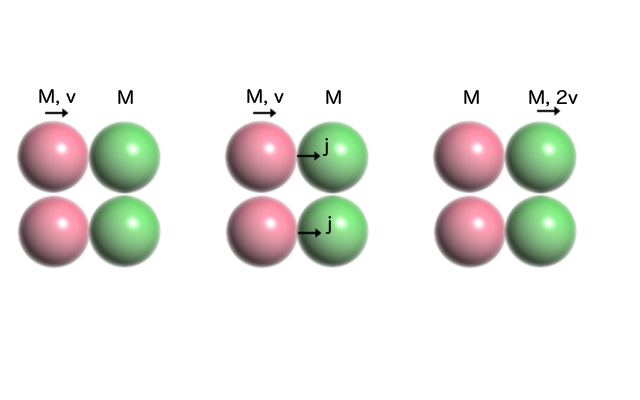
\includegraphics[width=0.8\linewidth]{fig/ballsNoMassSplit.png}
		\end{figure}
	\end{frame}

	%Display how mass-splitting will help the problem.
	\begin{frame}
		\frametitle{Spherical Voxelization}
		Mass Splitting, divide the impulse by the number of collisions
		\begin{figure}
			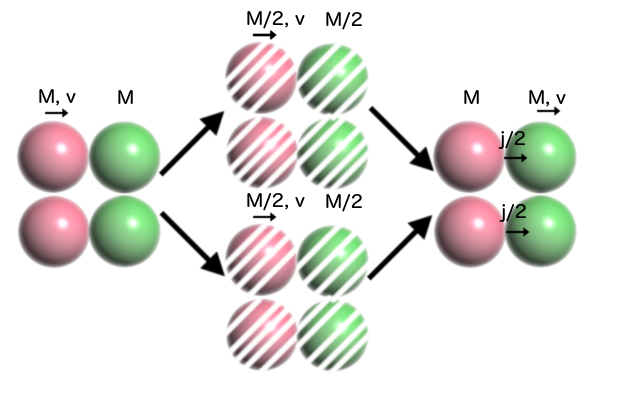
\includegraphics[width=0.6\linewidth]{fig/ballsMassSplit.png}
		\end{figure}
		We need to keep track of the number of collisions between each body pair
	\end{frame}

	\begin{frame}
		\frametitle{Parallelization of Impulses}
		\begin{columns}[c] % The "c" option specifies centered vertical alignment while the "t" option is used for top vertical alignment
			\column{.45\textwidth} % Left column and width
			\begin{itemize}
				\item Interpenetrations are solved by velocity biasing
			\end{itemize}

			\column{.5\textwidth} % Right column and width

			\begin{figure}
				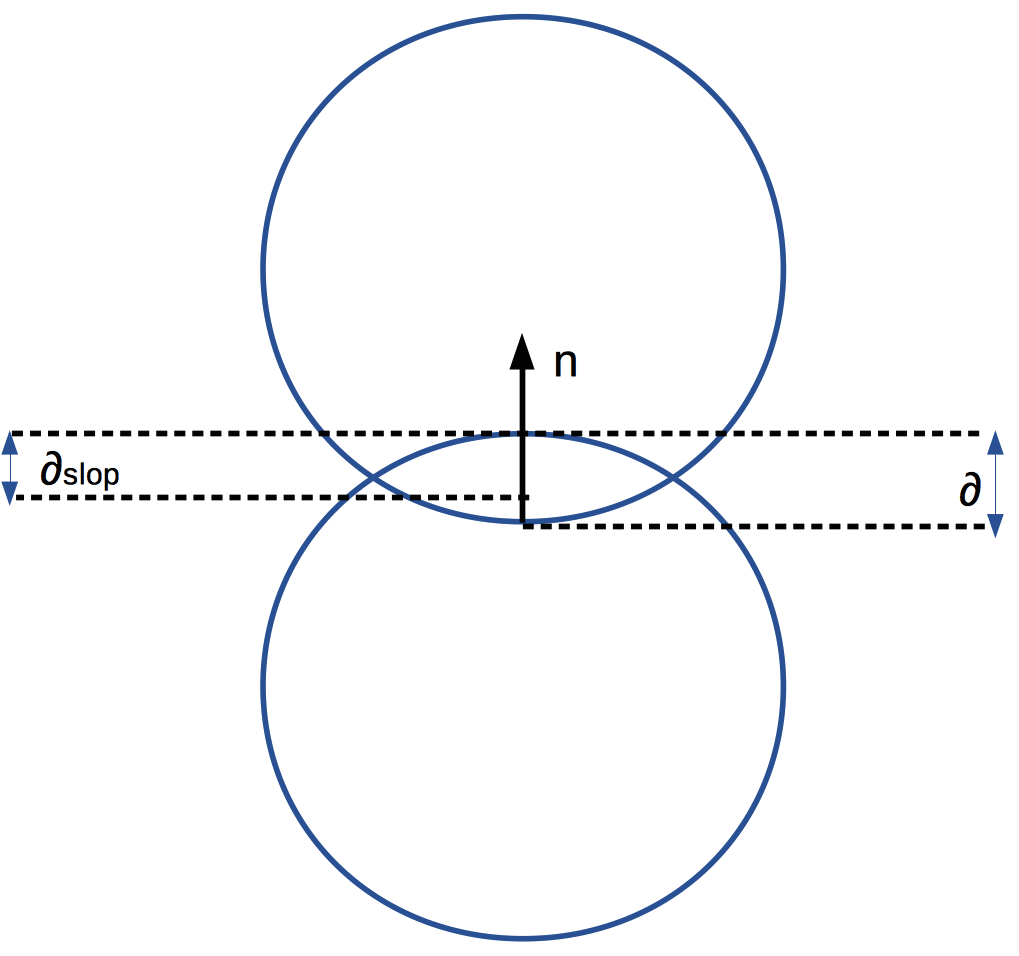
\includegraphics[width=0.8\linewidth]{fig/slop.png}
			\end{figure}

		\end{columns}
	\end{frame}


	\subsection{Collision detection}
	%Spatial partitioning grid
	\begin{frame}
		\frametitle{Spatial Partitioning}
		Uniform 3D grid for collision detection - Spatial Partioning\\
		\begin{figure}
			\includegraphics[width=0.3\linewidth]{fig/bins.png}
		\end{figure}
	\end{frame}

	%Sorting the particles along one dimension increases coherency
	\begin{frame}
		\frametitle{Spatial Partitioning}
		Reordering the particles during grid construction increases performance - coherent reads
		\begin{figure}
			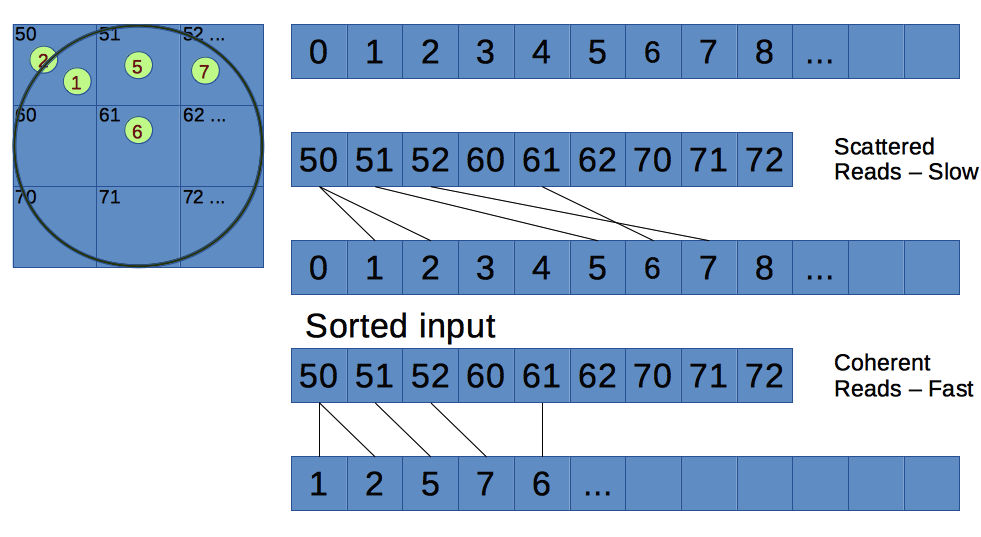
\includegraphics[width=0.7\linewidth]{fig/prefix1.png}
		\end{figure}
	\end{frame}

	%The particles are sorted through counting sort (prefix sums)
	\begin{frame}
		\frametitle{Spatial Partitioning}
		The particles are reordered using prefix sums\\
		\begin{figure}
			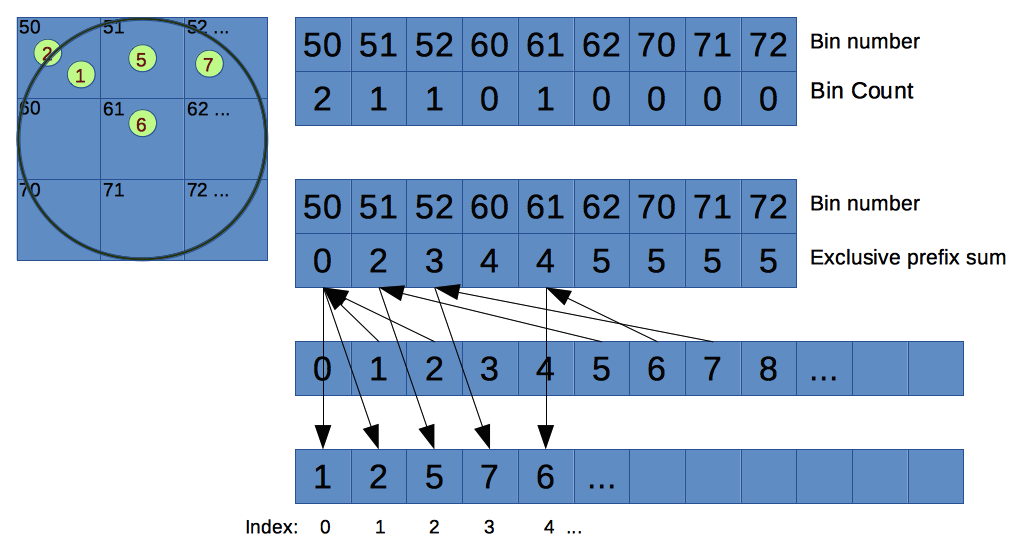
\includegraphics[width=0.7\linewidth]{fig/prefix2.png}
		\end{figure}
	\end{frame}

	\subsection{State update}
	% \begin{frame}
	% 	\frametitle{State update}
	% 		The impulses are transferred to the body \\
	% 		The total impulses are used for integration \\
	% 		The current physics pipeline on next slide
	% \end{frame}
	%Image of the current shader pipeline.

	\begin{frame}
		\frametitle{Current Pipeline}

		\begin{figure}
			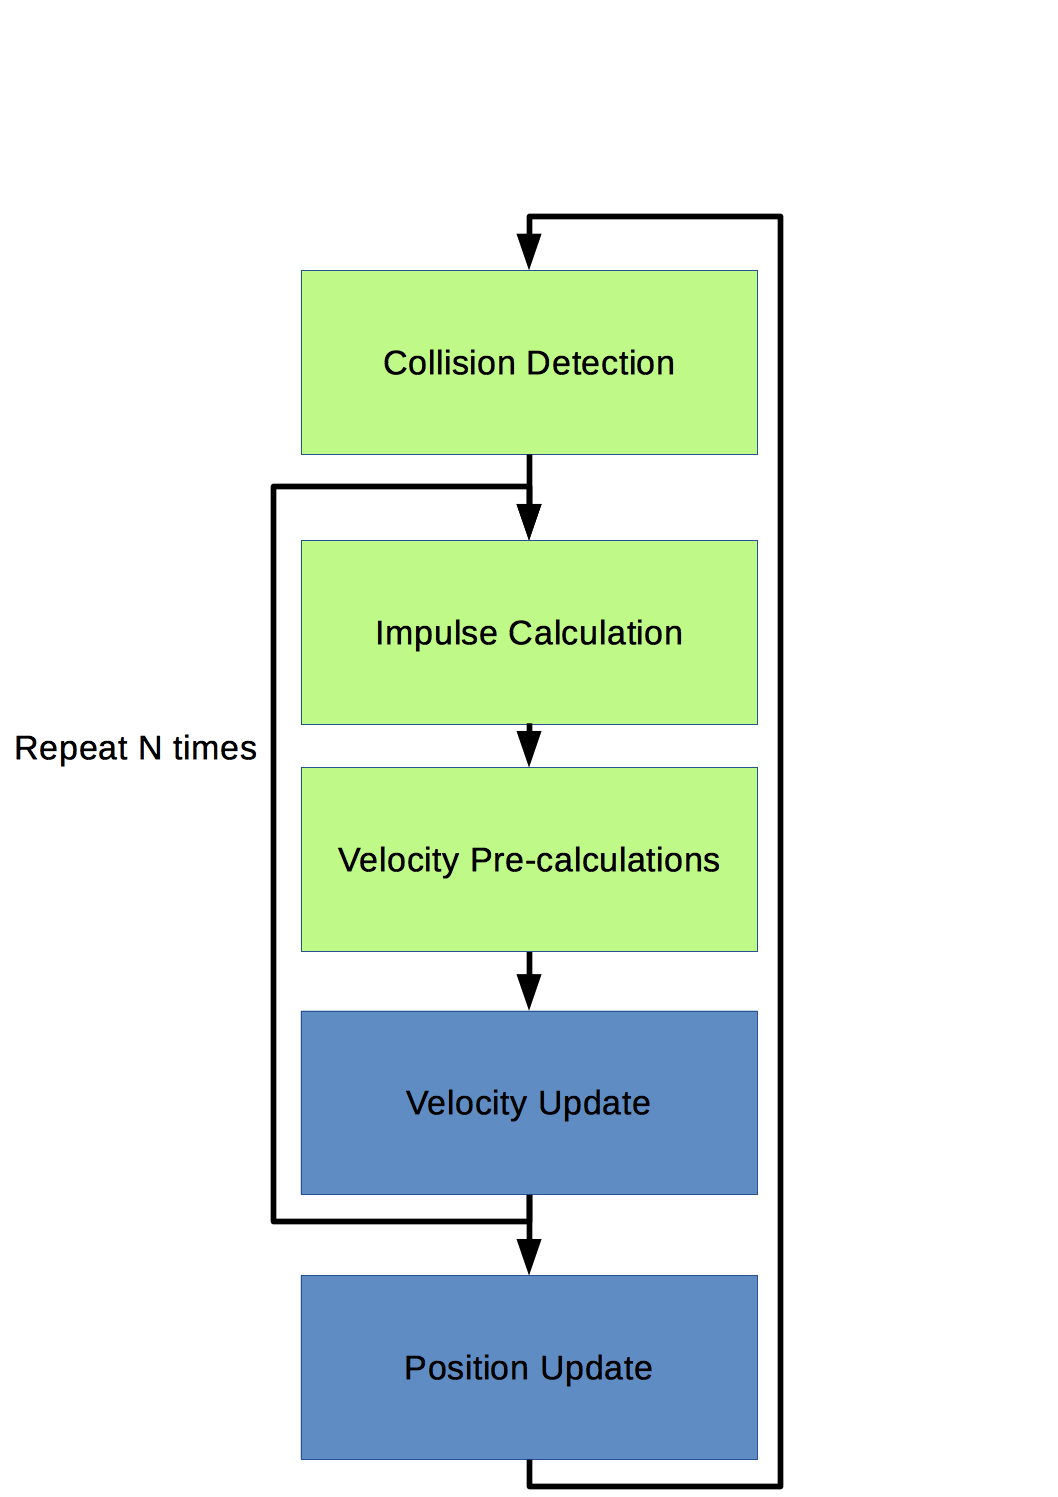
\includegraphics[width=0.45\linewidth]{fig/shaderflow2.png}
		\end{figure}
	\end{frame}

	\section{Improvements}
	\subsection{Modified Normals}
	\begin{frame}
		\frametitle{Modified Normals}
		\begin{itemize}
			\item Modify the normals to better approximate original surface
			\item Reduces the number of iterations needed to avoid tunneling
			\item In addition reduces tunneling effects
		\end{itemize}
	\end{frame}

	\subsection{Tightened Voxelization}
	\begin{frame}
		\frametitle{Tightened Voxelization}
		\begin{itemize}
			\item Move the spheres closer (overlapping) to better approximate original surface
			\item Reduces the number of iterations needed to avoid tunneling
			\item Performance hit in collision detection
		\end{itemize}
		Outperforms modified normals
	\end{frame}

	\begin{frame}
		\frametitle{Tightened Voxelization}
		\begin{figure}
			\includegraphics[width=0.8\linewidth]{fig/tightenedVoxels.png}
		\end{figure}
	\end{frame}

	\section{Results}
	\begin{frame}
		\frametitle{Results}
		\begin{figure}
			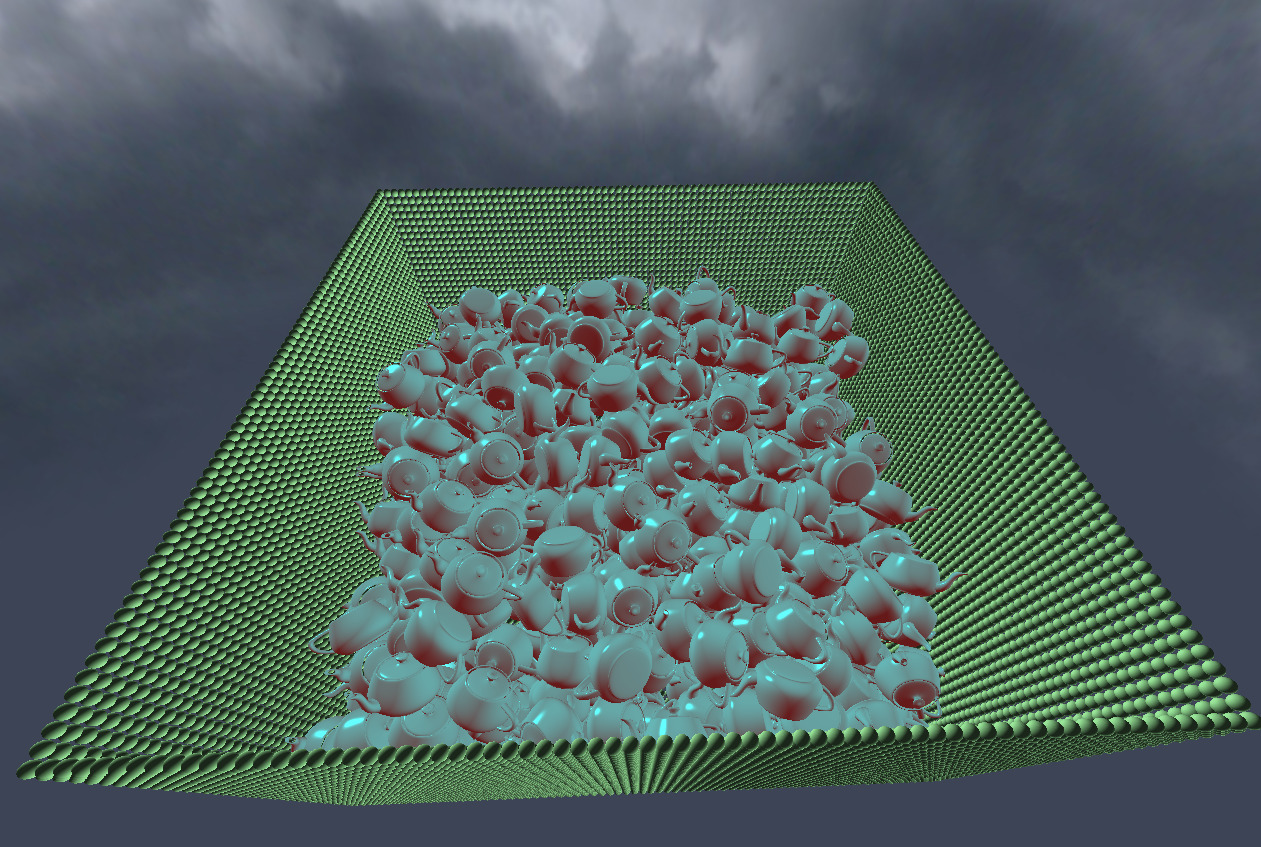
\includegraphics[width=0.6\linewidth]{fig/finishedSphoxTeapot.png}
		\end{figure}
	\end{frame}
	\begin{frame}
		\frametitle{Results}
		\begin{figure}
			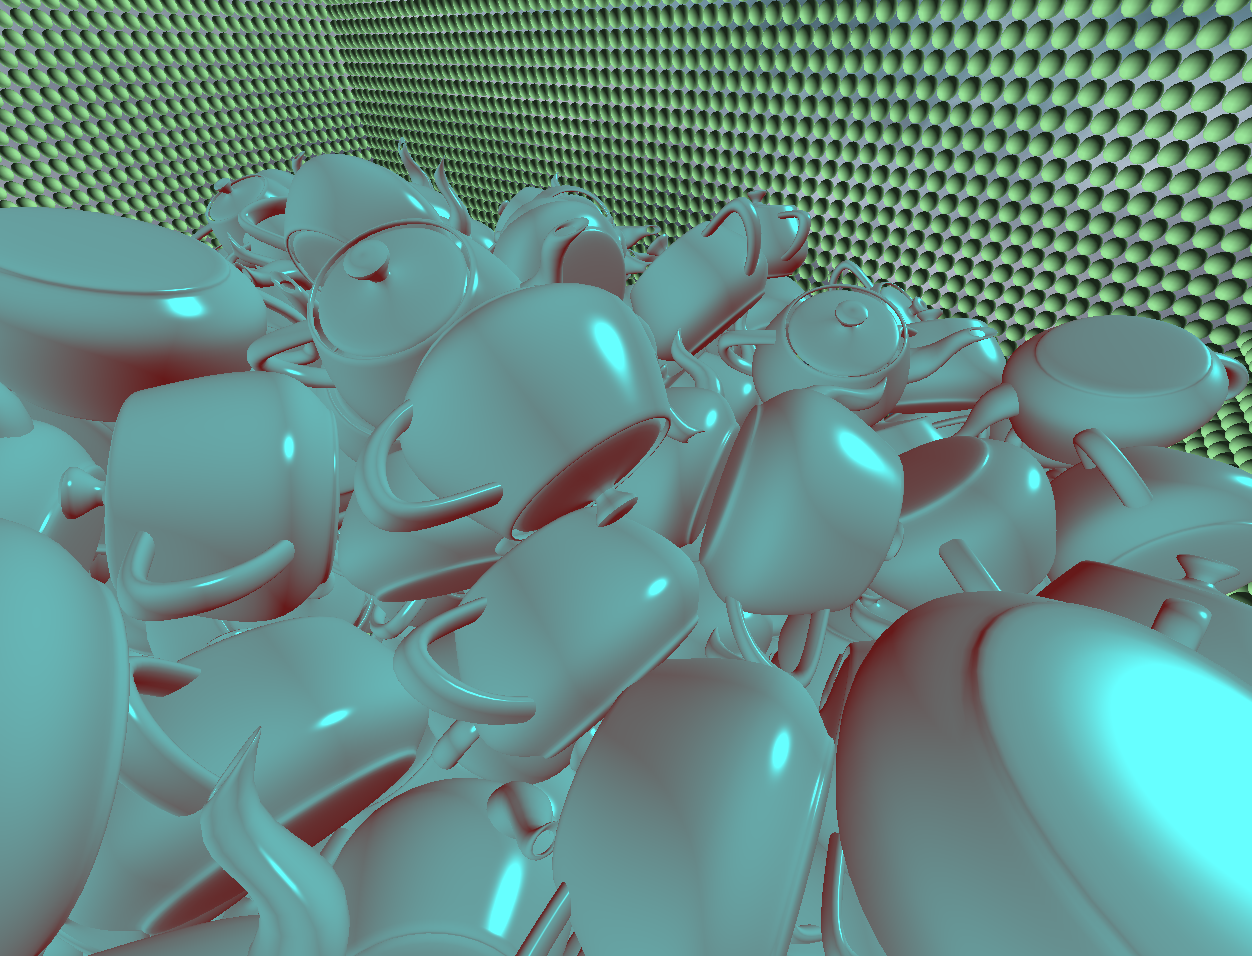
\includegraphics[width=0.6\linewidth]{fig/closeUpSphox.png}
		\end{figure}
	\end{frame}

	\begin{frame}
		\frametitle{Performance Comparison}
		\begin{figure}
			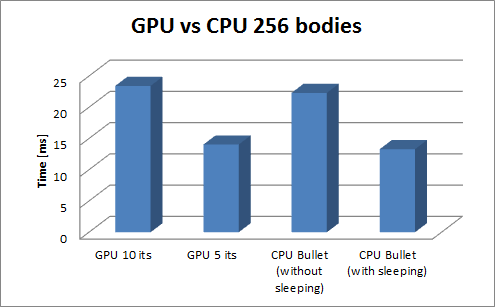
\includegraphics[width=0.6\linewidth]{fig/GvC256.png}
		\end{figure}
	\end{frame}
	\begin{frame}
		\frametitle{Performance Comparison}
		\begin{figure}
			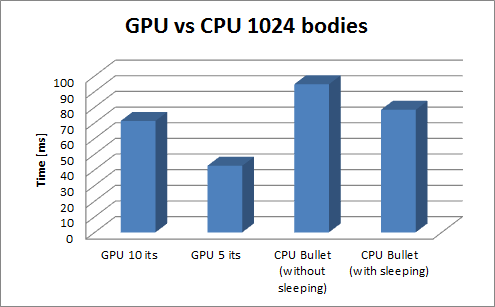
\includegraphics[width=0.6\linewidth]{fig/GvC1024.png}
		\end{figure}
	\end{frame}
	\section{Demo and Final remarks}
	\begin{frame}
		\frametitle{Final Remarks}
		\begin{itemize}
			\item Handles concave properties
			\item Runs fully on the GPU
			\item Performs comparable to Bullet 2.86 with low bodycount scenes
			\item Outperforms Bullet 2.86 with high bodycount scenes
			\item Many improvements left to implement
		\end{itemize}
	\end{frame}

	%------------------------------------------------

	% \begin{frame}[fragile] % Need to use the fragile option when verbatim is used in the slide
	% 	\frametitle{Citation}
	% 	An example of the \verb|\cite| command to cite within the presentation:\\~
	%
	% 	This statement requires citation \cite{p1}.
	% \end{frame}

	%------------------------------------------------

	% \begin{frame}
	% 	\frametitle{References}
	% 	\footnotesize{
	% 	\begin{thebibliography}{99} % Beamer does not support BibTeX so references must be inserted manually as below
	% 		\bibitem[Smith, 2012]{p1} John Smith (2012)
	% 		\newblock Title of the publication
	% 		\newblock \emph{Journal Name} 12(3), 45 -- 678.
	% 	\end{thebibliography}
	% 	}
	% \end{frame}

	%------------------------------------------------

	\begin{frame}
		\Huge{\centerline{Opposition followed by questions}}
	\end{frame}

	%----------------------------------------------------------------------------------------

\end{document}
